% Drawing 100/01-4 -- folder 100, batch 01, archive page 20 (PDF page 21).
% Transcription: sous le cadre, à gauche, un grand croquis : une région de la base $S$ balayée de courbes parallèles, avec, marqués sur elle, « $S$ », « $S_0$ » (fortement repassé), « $S_1 \leftarrow S'$ » et, au-dessus, « $A_{S'} \to B_{S'}$ » ; un point cerclé au coin inférieur gauche, où aboutit une flèche
% Kind: region of a base swept by parallel curves. Method 2 (schematic redraw from the facsimile). Status: ok.
% Notes: Redrawn on a tight crop. The region: a left side, a top edge (the long stroke under the boxed text, which here also closes the region), a right side turning into the lower right edge, and the bottom edge; six parallel curves sweep it up to the right, the first five starting on the bottom edge (at the corner and at four computed feet), the sixth starting on a transversal; four wavy transversal strokes cross them (one through S_0, one in the middle ending where the sixth curve starts, a short one ending at the end of the bottom edge, one at the right through B_S'). Marked on it: S, S_0 (heavily retraced, drawn bold), S_1 <- S' (heavy arrow), A_S' -> B_S' above; the ringed point below the lower left corner with the arrow ending at it. Left out: the text lines at the top and the vertical stroke at the upper left (frame of the box above). Still differs: the curves and wavy strokes are approximate, and whether the long upper stroke is the top of the region or the bottom of the frame is a reading. Redrawn 2026-11-09 (issue 128): to check again. Question settled by a machine pass on the facsimile, 2026-11-12 (page): the long upper stroke meets the left side of the box above at a corner, so it is the bottom of that frame; the region's left side starts below it and its right side rises to it, so the same stroke also bounds the region at the top, and it stays drawn where it is. Not checked by a reader. 2026-11-13, Claude Opus 5.5, overlay check (issue 147): not compiled (no TeX in the session); the TikZ rasterised and laid over the 350 dpi colour render of the scan, with an ink/pencil separation of the crop. Redrawn on the ink: the six curves through points read on them (the second, third and fourth were 2 to 3 units off in their middle); the sixth curve starts at the lower end of the short transversal, at about (71, 50.5), and not on the middle transversal (that one ends on the fifth curve); the lower right edge runs on to the head of the arrow from S'; S' placed on its glyph. Every element lies on the ink to within about 1 to 1.5 units (the lower parts of the first two curves are drawn about a unit left of their ink, within a stroke's width of the doubled pencil). Left out: the text lines at the top and the strokes of the box above (its left side and the oblique stroke). The long upper stroke is both the bottom of that box and the top of the region, as settled on 2026-11-12.
% Coordinates: 1 unit = 1 mm = 1/100 of the crop width (bbox in page fractions: [0.08, 0.25, 0.56, 0.47]).
% Redrawn by Claude (claude-opus-5-5), issue #73, 2026-11-09; not checked by a human; not compiled (no TeX in the session).
% Revised by Claude Opus 5.5 (claude-opus-5-5), issue #147, 2026-11-13: overlay check on the colour scan; not checked by a human; not compiled (no TeX in the session).
% Rights: reproduces part of the work -- behind RENDER_TRANSCRIPTS, never published by itself.
\documentclass[tikz,border=3pt]{standalone}
\usepackage{amsmath,amssymb}
\usetikzlibrary{patterns,arrows.meta}
\tikzset{pencil/.style={black!45}, struck/.style={black!35}, mark/.style={circle,draw,inner sep=1.3pt}, pt/.style={circle,fill,inner sep=0.9pt}, opt/.style={circle,draw,fill=white,inner sep=1.1pt}}
\begin{document}
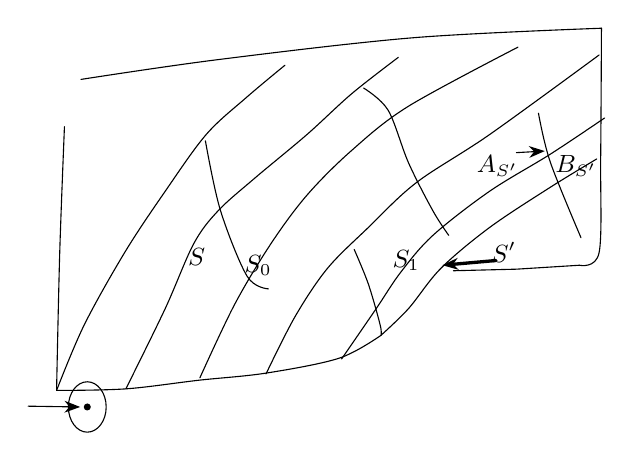
\begin{tikzpicture}[x=1mm,y=1mm,line cap=round,line join=round,font=\scriptsize]
\draw plot[smooth, tension=0.55] coordinates {(30.6,-24) (30,-40) (29.6,-57.5)};
\draw plot[smooth, tension=0.55] coordinates {(32.7,-18) (50,-15.5) (75,-12.7) (98.8,-11.5)};
\draw plot[smooth, tension=0.55] coordinates {(98.8,-11.5) (98.7,-28) (98.5,-40) (96,-41.6)};
\draw (96,-41.6) -- (88,-42.1) -- (80,-42.3);
\draw plot[smooth, tension=0.55] coordinates {(29.6,-57.5) (38.4,-57.3) (47.7,-56.2) (56.2,-55.3) (65.5,-53.4) (70.8,-50.5)};
\draw plot[smooth, tension=0.55] coordinates {(29.6,-57.5) (33.1,-49.2) (38.3,-39.9) (43.4,-32.2) (48.6,-25) (53.7,-20.3) (58.6,-16.2)};
\draw plot[smooth, tension=0.55] coordinates {(38.4,-57.3) (43.4,-47.1) (47,-38.9) (50.1,-34.7) (54.7,-30.6) (61.4,-25) (67.1,-19.8) (73,-15.2)};
\draw plot[smooth, tension=0.55] coordinates {(47.8,-55.9) (52.2,-46.6) (56.8,-38.9) (61.4,-32.7) (67.1,-27) (74.3,-21.4) (88.2,-13.9)};
\draw plot[smooth, tension=0.55] coordinates {(56.2,-55.4) (59.9,-48.1) (64,-42) (69.2,-36.8) (75.3,-31.1) (84.6,-25) (98.5,-14.9)};
\draw plot[smooth, tension=0.55] coordinates {(65.8,-53.5) (70.2,-47.1) (73.3,-42.5) (77.4,-37.8) (84.6,-32.2) (92.3,-27.5) (99.2,-22.9)};
\draw plot[smooth, tension=0.55] coordinates {(70.8,-50.5) (74.3,-47.1) (78.4,-42) (84.6,-36.8) (92.3,-31.7) (98.2,-28.1)};
\draw plot[smooth, tension=0.55] coordinates {(48.5,-25.8) (50.4,-34.6) (53.8,-43) (56.5,-44.6)};
\draw plot[smooth, tension=0.55] coordinates {(68.6,-19.1) (71.7,-21.9) (74.3,-28.6) (77.4,-34.7) (79.4,-37.8)};
\draw plot[smooth, tension=0.55] coordinates {(67.4,-39.6) (69.2,-44) (70.7,-49.2) (70.8,-50.5)};
\draw plot[smooth, tension=0.55] coordinates {(90.8,-22.3) (92.3,-28.5) (96.2,-38.1)};
\node[inner sep=1pt] at (47.4,-40.6) {\small $S$};
\node[inner sep=1pt,very thick] at (55.2,-41.6) {\small $S_0$};
\node[inner sep=1pt] at (74,-41) {\small $S_1$};
\draw[very thick,-{Stealth[length=2mm]}] (85.4,-41) -- (78.6,-41.6);
\node[inner sep=1pt] at (86.4,-40) {\small $S'$};
\node[inner sep=1pt] at (85.6,-29) {\small $A_{S'}$};
\draw[-{Stealth[length=2mm]}] (88,-27.3) -- (91.6,-27.1);
\node[inner sep=1pt] at (95.6,-29) {\small $B_{S'}$};
\draw (33.5,-59.6) ellipse[x radius=2.4, y radius=3.2];
\node[pt] at (33.5,-59.6) {};
\draw[-{Stealth[length=2mm]}] (26,-59.5) -- (32.6,-59.6);
\end{tikzpicture}
\end{document}
